\begin{document}
	\chapter{Results}
	
	The study conducted over the gathered data served for the definition of new metrics to measure the performance and robustness of the Lightning Network and for the formal modeling of two mathematical representation of the Lightning Network, from a static and dynamic point of view. The analysis is carried over a period of one month, one snapshot per day; this observation period will be justified by the results obtained by the analysis of daily behavior of the network that will be shown next.
	
	\section{Trends}
	
	The following section takes in consideration the most relevant trends of the network which are the nodes and edges variation, the average degree and the diameter of the network on a daily and a monthly basis. The analysis carried over the daily basis data is made to justify the decision of the focus on a larger time window. The reasons behind the following churn rates are out of the scope of this work, but it is likely that they largely depends on protocol changes, client errors and, possibly the popularity of the network itself.
	
	A full day representation of the Lightning Network consists of 144 snapshots taken at 10 minutes intervals; the 10 minutes intervals were chosen because every channel that is added (or removed) from the network must wait for the funding transaction (settlement transaction in case a channel is being closed) to be included in a block and added to the chain by the miners. The following results matched the expectation because, as stated in the white paper, a Lightning node and its channels are meant to have a long lifespan. The data refers to the date of May 16th, May 21th, May 26th, June 2nd, 
	
	\subsection{Daily nodes variation}
	
	\begin{figure}[h]
		\centering
		\begin{subfigure}{0.45\textwidth}
			\centering
			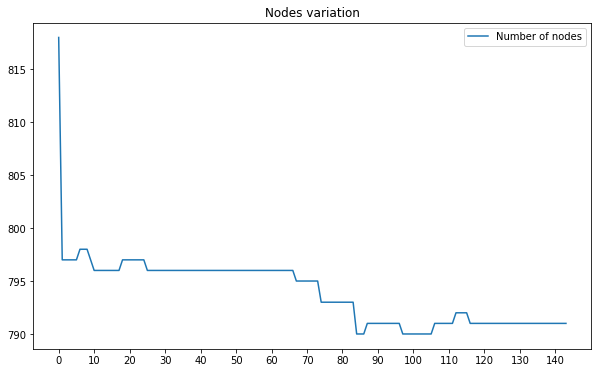
\includegraphics[width=\linewidth]{daily_number_of_nodes0}
			\caption{Snapshot, May 16th}
			\label{daily_node0}
		\end{subfigure}
		\begin{subfigure}{0.45\textwidth}
			\centering
			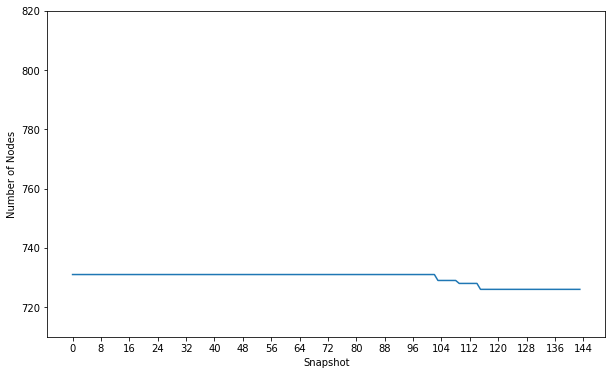
\includegraphics[width=\linewidth]{daily_number_of_nodes1}
			\caption{Snapshot, May 21th}
			\label{daily_node1}
		\end{subfigure}
			\begin{subfigure}{0.45\textwidth}
			\centering
			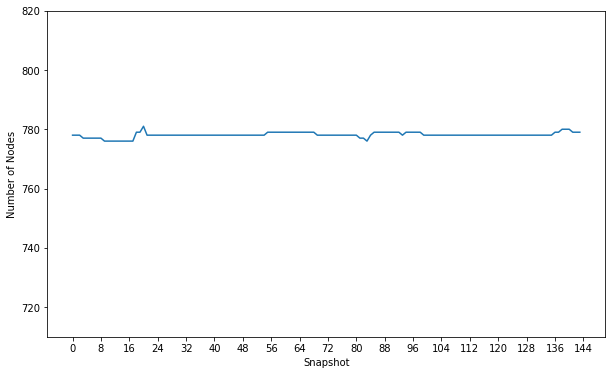
\includegraphics[width=\linewidth]{daily_number_of_nodes2}
			\caption{Snapshot, May 26th}
			\label{daily_node2}
		\end{subfigure}
		\begin{subfigure}{0.45\textwidth}
			\centering
			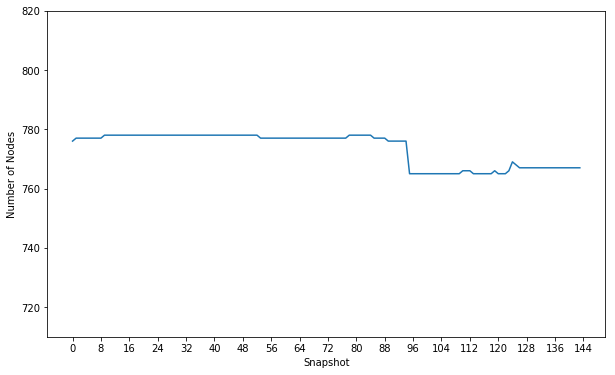
\includegraphics[width=\linewidth]{daily_number_of_nodes3}
			\caption{Snapshot, June 2nd}
			\label{daily_node3}
		\end{subfigure}
		
		\caption{Nodes trends on a daily basis}
		\label{daily_nodes_variation}
	\end{figure}

	Details on nodes variations on a daily basis are reported in \ref{daily_nodes_variation}. The figure shows the 144 snapshot of the network for four different days. We can notice a similar behavior between the snapshots pictured in (\ref{daily_node1}) and (\ref{daily_node3}), although we can't appreciate the same behavior in (\ref{daily_node0}) or (\ref{daily_node2}). 
	
	While the plots may present steep slopes, it has to be noticed that the number of nodes that are joining or leaving the network is actually very low. To figure out better the numbers, the following table will show the percentage variation with respect to the initial state of the network and the highest and lowest order the graph reached that day.
	
	\begin{center}
		\begin{tabulary}{\linewidth}{| L | C | C | C | C |}
			\hline
			 & May 16th (\ref{daily_node0}) & May 21th (\ref{daily_node1}) & May 26th (\ref{daily_node0}) & June 2nd (\ref{daily_node3}) \\
			\hline
			Starting nodes & 818 & 731 & 778 & 776 \\ \hline
			Final nodes & 791 & 726 & 779 & 767 \\ \hline
			Variation(\%) & -3.30\% & -0.68\% & +0.12\% & -1.15\% \\ \hline
			Max number of nodes & 818 & 731 & 781 & 778 \\ \hline
			Min number of nodes & 790 & 726 & 776 & 765 \\ \hline

		\end{tabulary}
	\end{center}
	
	\subsection{Daily edges variation}

	\begin{figure}[h]
		\centering
		\begin{subfigure}{0.45\textwidth}
			\centering
			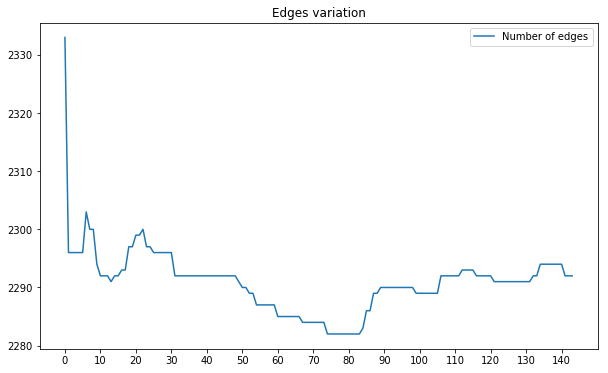
\includegraphics[width=\linewidth]{daily_number_of_edges0}
			\caption{Snapshot, May 16th}
			\label{daily_edges0}
		\end{subfigure}
		\begin{subfigure}{0.45\textwidth}
			\centering
			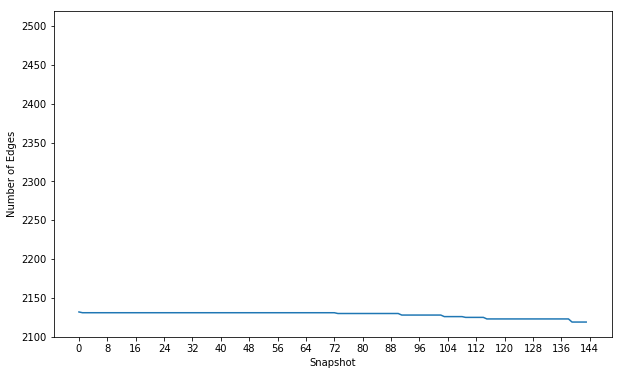
\includegraphics[width=\linewidth]{daily_number_of_edges1}
			\caption{Snapshot, May 21th}
			\label{daily_edges1}
		\end{subfigure}
		\begin{subfigure}{0.45\textwidth}
			\centering
			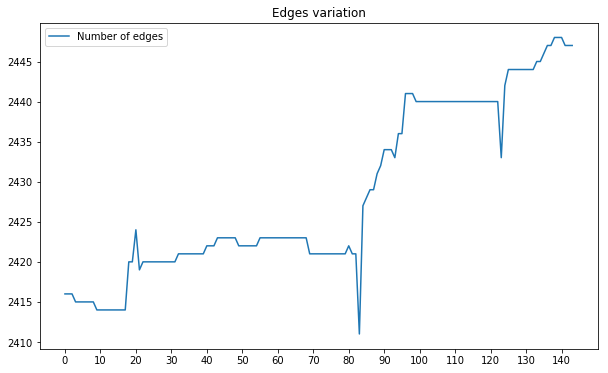
\includegraphics[width=\linewidth]{daily_number_of_edges2}
			\caption{Snapshot, May 26th}
			\label{daily_edges2}
		\end{subfigure}
		\begin{subfigure}{0.45\textwidth}
			\centering
			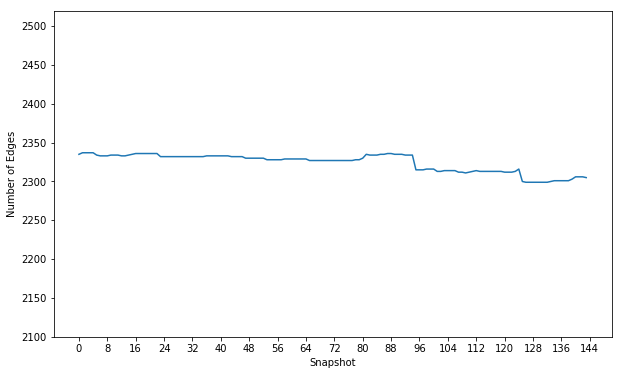
\includegraphics[width=\linewidth]{daily_number_of_edges3}
			\caption{Snapshot, June 2nd}
			\label{daily_edges3}
		\end{subfigure}
		
		\caption{Edges trends on a daily basis}
		\label{daily_edges_variation}
	\end{figure}

	The trends for edges essentially follow the same behavior of the nodes. It is trivial to see that for each node connecting (disconnecting) to the network, at least one channel is added (removed). The actual number of edges per node will be shown in the next section.
	
	\begin{center}
	\begin{tabulary}{\linewidth}{| L | C | C | C | C |}
		\hline
		& May 16th (\ref{daily_edges0}) & May 21th (\ref{daily_edges1}) & May 26th (\ref{daily_edges0}) & June 2nd (\ref{daily_edges3}) \\
		\hline
		Starting edges & 2333 & 2132 & 2416 & 2335 \\ \hline
		Final edges & 2292 & 2119 & 2447 & 2305 \\ \hline
		Variation(\%) & -1.75\% & -0.60\% & +1.28\% & -1.28\% \\ \hline
		Max num. edges & 2333 & 2132 & 2448 & 2337 \\ \hline
		Min num. edges & 2282 & 2119 & 2411 & 2299 \\ \hline	
	\end{tabulary}
	\end{center}

	\subsection{Daily average degree variation}

	\begin{figure}[h]
	\centering
		\begin{subfigure}{0.45\textwidth}
			\centering
			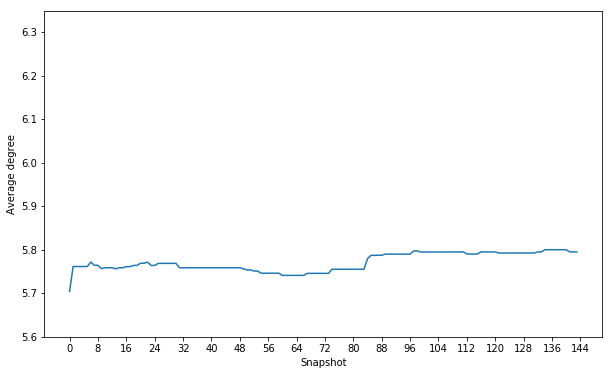
\includegraphics[width=\linewidth]{daily_average_degree0}
			\caption{Snapshot, May 16th}
			\label{daily_degree0}
		\end{subfigure}
		\begin{subfigure}{0.45\textwidth}
			\centering
			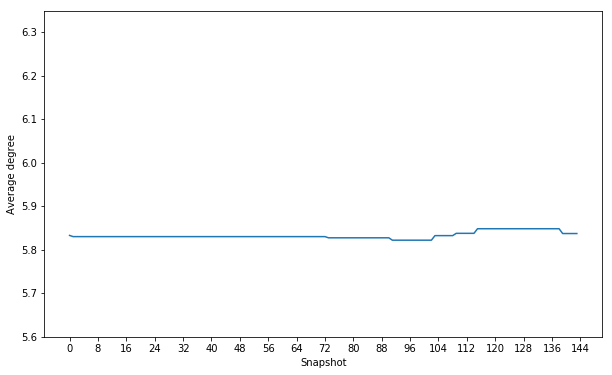
\includegraphics[width=\linewidth]{daily_average_degree1}
			\caption{Snapshot, May 21th}
			\label{daily_degree1}
		\end{subfigure}
		\begin{subfigure}{0.45\textwidth}
			\centering
			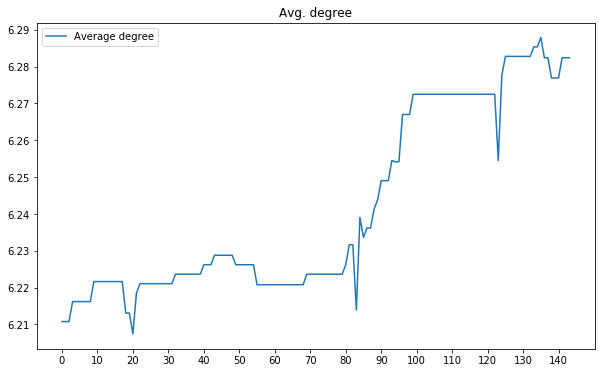
\includegraphics[width=\linewidth]{daily_average_degree2}
			\caption{Snapshot, May 26th}
			\label{daily_degree2}
		\end{subfigure}
		\begin{subfigure}{0.45\textwidth}
			\centering
			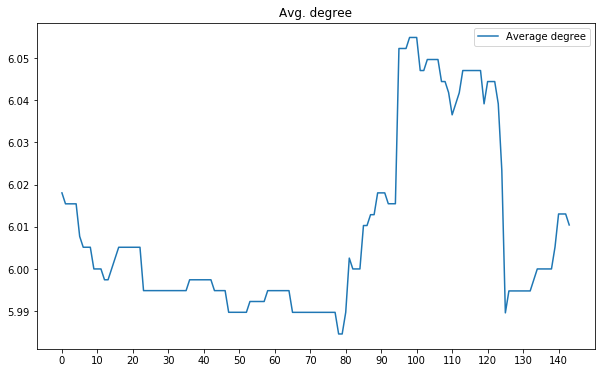
\includegraphics[width=\linewidth]{daily_average_degree3}
			\caption{Snapshot, June 2nd}
			\label{daily_degree3}
		\end{subfigure}
	
	\caption{Average degree on a daily basis}
	\label{daily_degree _variation}
	\end{figure}

	The daily average degree score appears to be confined between an all time highest of 1.59\% and -0.12\% among the days in exam and it is coherent with the number of nodes and edges fluctuation. By putting in relation the number of nodes and average degree variation it is possible to learn more about what kind of nodes are joining or leaving the network: for example data from (\ref{daily_node0}) and (\ref{daily_edges0}) show a negative edges and nodes fluctuation while the average degree variation of (\ref{daily_degree0}) is overall increased, suggesting that the nodes that left the network were actually single-channels node.


	\begin{center}
		\begin{tabulary}{\linewidth}{| L | C | C | C | C |}
			\hline	
			& May 16th (\ref{daily_degree0}) & May 21th (\ref{daily_degree1}) & May 26th (\ref{daily_degree2}) & June 2nd (\ref{daily_degree3}) \\
			\hline
			Starting degree & 5.70 & 5.833 & 6.21  & 6.018 \\ \hline
			Final degree & 5.79 & 5.837 & 6.28 & 6.010 \\ \hline
			Variation (\%) & +1.59\% & +0.07\% & +1.15\% & -0.12\% \\ \hline
			Max avg. degree & 5.80 & 5.84 & 6.28 & 6.05 \\ \hline
			Min avg. degree & 5.70 & 5.82 & 6.20 & 5.98 \\ \hline		
		\end{tabulary}
	\end{center}
	
	\subsection{Daily diameter}
	
		\begin{figure}[h]
		\centering
		\begin{subfigure}{0.45\textwidth}
			\centering
			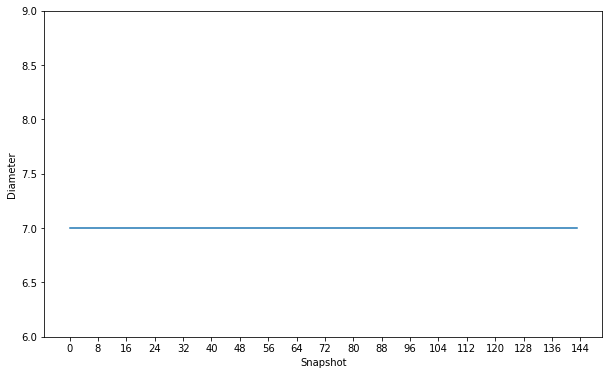
\includegraphics[width=\linewidth]{daily_diameter0}
			\caption{Snapshot, May 16th}
			\label{daily_diameter0}
		\end{subfigure}
		\begin{subfigure}{0.45\textwidth}
			\centering
			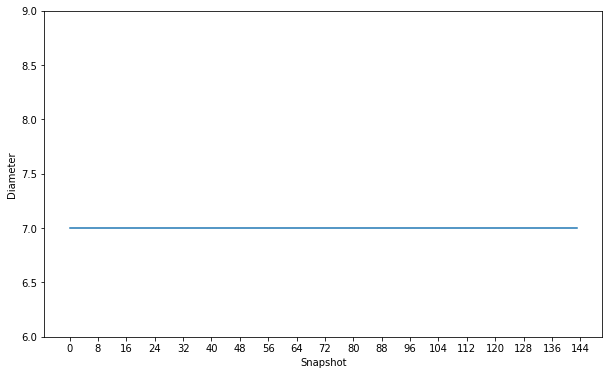
\includegraphics[width=\linewidth]{daily_diameter1}
			\caption{Snapshot, May 21th}
			\label{daily_diameter1}
		\end{subfigure}
		\begin{subfigure}{0.45\textwidth}
			\centering
			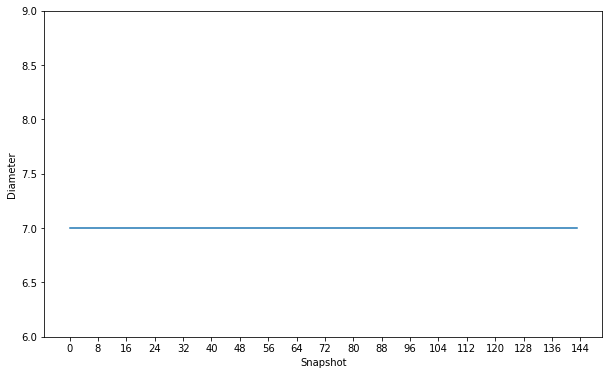
\includegraphics[width=\linewidth]{daily_diameter2}
			\caption{Snapshot, May 26th}
			\label{daily_diameter2}
		\end{subfigure}
		\begin{subfigure}{0.45\textwidth}
			\centering
			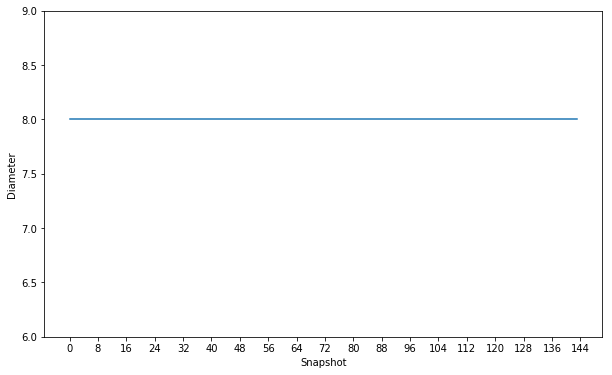
\includegraphics[width=\linewidth]{daily_diameter3}
			\caption{Snapshot, June 2nd}
			\label{daily_diameter3}
		\end{subfigure}
		
		\caption{Diameter trends on a daily basis}
		\label{daily_diameter}
	\end{figure}
	
	The graph diameter is a measures that is derived from the wider notion of \textit{eccentricity} $\epsilon$ which is defined as the greatest shortest distance between a vertex \(v\) and every other vertex and expresses how much a node \(v\) is distant from the farthest node of the graph. The diameter \(d\) is the greatest shortest path among all the pair of nodes, i.e. it is the maximum eccentricity of any vertex in the graph.
	
	\[d = \max_{v \in V} \epsilon(v)\]
	
	The churn rate of the network in all four snapshots is too low to justify a variation, resulting in a constant behavior along the 144 snapshots. These trends were actually showed to justify a wider period of observation as it is hard to infer any properties from the gathered data. In the following sections, the very same trends will be showed with respect to a 32 days period. 

	\subsection{Monthly nodes variation}
	
	\begin{figure}
		\centering
		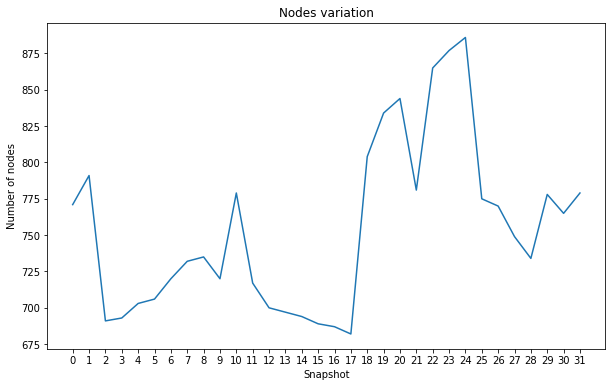
\includegraphics[width=\linewidth]{number_of_nodes}
		\caption{Monthly nodes variation.}
		\label{monthly_nodes}
	\end{figure}
	
	Figure \ref{monthly_nodes} displays the trend of the churning nodes from May 15th to June 27th. Differently from what has been observed on the daily trends, here the overall variation at the end of the observation period is, as expected, more pronounced as the size of the network has seen a +13.73\% joining rate.
	
	\begin{center}
		\begin{tabulary}{\linewidth}{| L | C | C | C | C | C |}
			\hline	
			& Starting nodes & Final nodes  & Variation(\%) & Max num. of nodes & Min num. of nodes \\ \hline
			May 15th - June 27th & 779 & 886 & +13.73\% & 886 & 682 \\ \hline
		\end{tabulary}
	\end{center}
	
	\subsection{Monthly edges variation}
	\begin{figure}
		\centering
		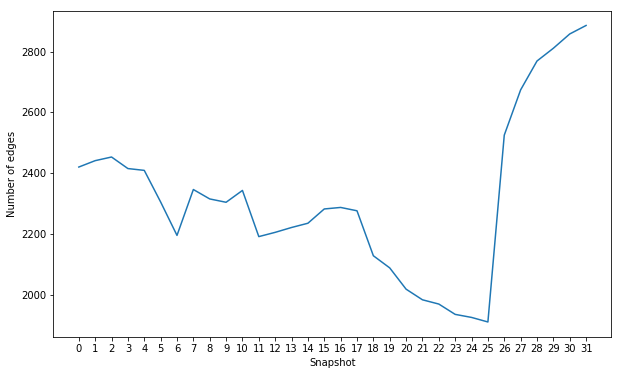
\includegraphics[width=\linewidth]{number_of_edges}
		\caption{Monthly edges variation.}
		\label{monthly_edges}
	\end{figure}

	Edges trend follow the same nodes trend as it has been already showed with the daily trends. Here the gap between highs and lows is even more pronounced because, trivially, it is likely that nodes have more than one channel towards other nodes and this is reflected by the variation observed with respect to the nodes, being it +19.25\%. This graph helps to understand better the dynamic nature of the Lightning Network channels, as the churning rate of edges is higher than the one accounting for the nodes. 
	
	\begin{center}
		\begin{tabulary}{\linewidth}{| L | C | C | C | C | C |}
			\hline	
			& Starting channels & Final channels  & Variation(\%) & Max num. of channels & Min num. of channels \\ \hline
			May 15th - June 27th & 2420 & 2886 & +19.25\% & 2886 & 1910 \\ \hline
		\end{tabulary}
	\end{center}
	
	\subsection{Monthly average degree variation}
	
	\begin{figure}
		\centering
		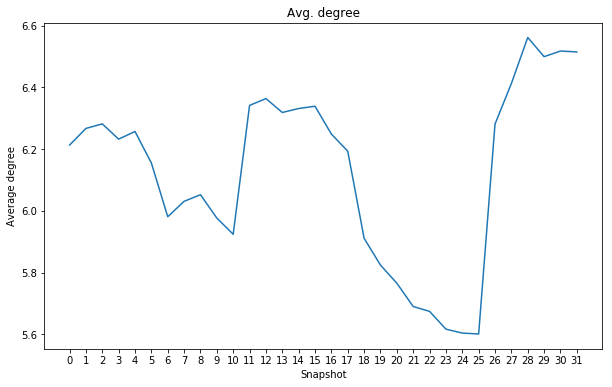
\includegraphics[width=\linewidth]{average_degree}
		\caption{Monthly average degree.}
		\label{monthly_degree}
	\end{figure}
	
	As a consequences for these rates, the average degree of the network oscillates between a higher gap with respect to what has been observed during the daily analysis where the fluctuation was on average +0,67\%. Later it will be showed the actual degree distribution of the graph, and an interesting property that will emerge is that it resembles a power-law distribution. Thanks to this intuition it will be possible to play around this feature in the building of an equivalent model. The following table shows the main characteristics emerged from the overall average degree analysis.
	
	\begin{center}
		\begin{tabulary}{\linewidth}{| L | C | C | C | C | C |}
			\hline	
			& Starting degree (avg.) & Final degree (avg.)  & Variation(\%) & Max avg.degree & Min avg. degree \\ \hline
			May 15th - June 27th & 6.21 & 6.51 & +4.85\% & 6.56 & 5.60 \\ \hline
		\end{tabulary}
	\end{center}
	
	\subsection{Monthly diameter}
	
	The diameter essentially falls within the already known bounds found during their analysis over a daily time window, although, thanks to a wider observation period, it is possible to see how frequent the oscillation between different diameters are. In the case in exam, the plot shows a period in which the network has seen an increase that lasted for 22 days. the importance of this data will be better explained in the next session, but shortly, if a payment uses the geodesic distance as the preferred method to deliver funds, then it would mean that in the worst case there is the need to cross 7 (or 8) channels before reaching the desired peer. Keeping track of this feature may help to balance the network in a way so that new channels can fill the gap between less connected clusters or to be aware of failures of central nodes.
	
	\begin{figure}
		\centering
		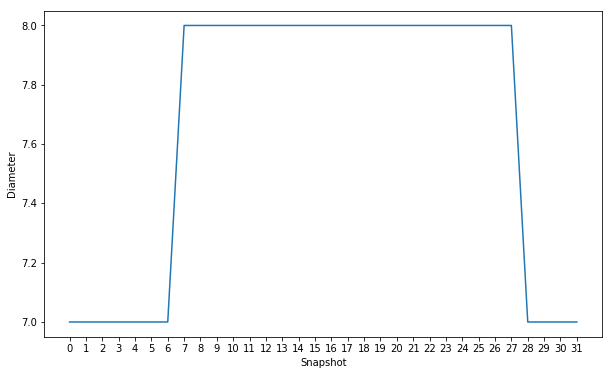
\includegraphics[width=\linewidth]{distance}
		\caption{Diameter.}
		\label{monthly_diameter}
	\end{figure}

	\section{Betwenness	centrality}
	\label{sec:betweenness}
	
	The betweenness centrality is a measure of centrality in graph theory based on shortest paths and it was first formalized in 1977 by Freeman, L.\cite{Freeman1977}. The betweenness centrality indicates how much a node in a graph stand between each other shortest paths, and it is a fundamental tool to evaluate the importance of nodes in several fields: for example, in telecommunication systems, a node with a high betweenness centrality means that a large portion of the traffic passes through it, that is, it effectively controls an appreciable part of the network but it also finds applications in biology, social networks, transport networks and many other research fields. 
	
	Since the Lightning Network is a peer-to-peer payment system, it is crucial to understand which are the main players involved as they fulfill the role of bridges of different parts of the network (thus, their disconnection may cause a temporary denial of service) and entry points for new nodes as they offer guarantees over their reliability given the fact that they already manage a high payment traffic (also known as \textit{preferential attachment} property from scale-free network), essentially forming the real backbone of the Lightning Network. But before proceeding with the results of the betweenness centrality measurements it is necessary to talk about the metric chosen to evaluate the shortest path.
	
	The Lightning Network is a payment system based on routes between peers that delegates the payment task to their neighbors thanks to a special contract called HTLC. However, it may happen that a fund that is being processed may end up kept in hostage by a faulty node; therefore, in order to prevent this disruptive scenario a timelock (namely nLockTime parameter) is applied for each HTLC transactions that occur during the payment in order to have the certainty that, after a fixed amount of time, the payment can be considered valid. The best case scenario occurs when all the nodes of a payment path are cooperative and fulfill their duties (i.e. the payment is resolved almost instantly), while the worst case scenario occurs when each node acts maliciously by waiting until the expiration date of the HTLC approaches and then fulfilling their task, as the fidelity bonds between two parties enforce to adhere to the protocol (penalty, the lose of all the liquidity in the channel in favor of the offended party). 
	
	By default, the nLockTime parameter is set to 144 blocks which are approximately 24 hours (the Bitcoin blockchain can be seen as a timestamp service, hence the two expressions are mutual) and we've seen so far that the diameter of the network is around 7 and 8 as showed in Figure \ref{monthly_diameter}. Thus, if the path between two peers has only malicious participant it would mean that a transactions can be considered valid only if 7 days are passed, and the funds gets locked out as well. This is the reason why it is advised to pay only for small amounts of Bitcoins, as larger sums could be locked for several days as they are still considered involved in an open payment operation: if the same situation should happen with larger sums, the consequences would be disruptive for the network as it may prevent peers to fulfill any payment for days; another reason for small payments is that large transfers of money would drain a channel balance instantly, forcing the settlement of the channel after few transactions. A new approach to payments called AMP \cite{Amp2018} - Atomic Multipaths Payment - has been proposed as a workaround to the latter problem. It should be clear to the reader then that a payer has the necessity to minimize the distance between him and his payee, as it will minimize the time required to process a transaction in case of adversarial nodes along the path and also will minimize the time he has to wait before getting his channel funds unlocked and ready to use for a new transaction.
	
	It has been observed that more than 90\% of nodes policies carried the default timelock delta value of 144. Since the analysis was carried on the testnet environment it is probable that the policies of the remaining 10\% of the edges were modified for research activities since the Lightning Network authors strongly suggest to stick with the default value for safety reason. After having removed all the edges whose timelock was different from 144, it was safe to assume that the traversal cost of an edge was equal to 1 without loss of generality.
	
	As for the algorithm itself that will be used, the Networkx has its own implementation based on the Ulrik Brandes \cite{Brandes2001} variant that computes the betweenness centrality running in $\theta(nm)$ and $\theta(n + m)$ space where $n$ is the number of nodes and $m$ the number of edges whereas the fastest known algorithm at the time required $\theta(n^3)$ time and $\theta(n^2)$ space.	Generally speaking, the betweenness centrality is evaluated according to the formula 
	\begin{equation}
		g(v) = \sum_{s \neq v \neq t}{\frac{\sigma_{st}(v) }{\sigma_st}}
	\end{equation}
	where $\sigma_st$ is the total number of shortest paths from node $s$ and node $t$ and $\sigma_{st}(v)$ is the number of paths that pass through $v$. In order to have $g(v) \in [0, 1]$ it is necessary to normalize the values by dividing (for undirected graphs) by $(N-1)(N-2)/2$ where $N$ is the total number of nodes.

	\begin{figure}
		\centering
		\begin{subfigure}{0.45\textwidth}
			\centering
			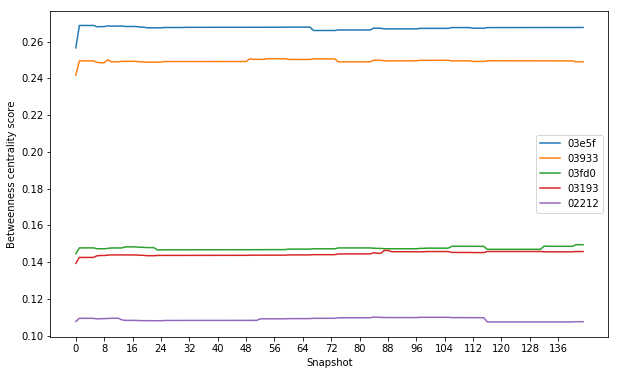
\includegraphics[width=\linewidth]{daily_betweenness_centrality0}
			\caption{Snapshot, May 16th}
			\label{daily_beetwenness0}
		\end{subfigure}
		\begin{subfigure}{0.45\textwidth}
			\centering
			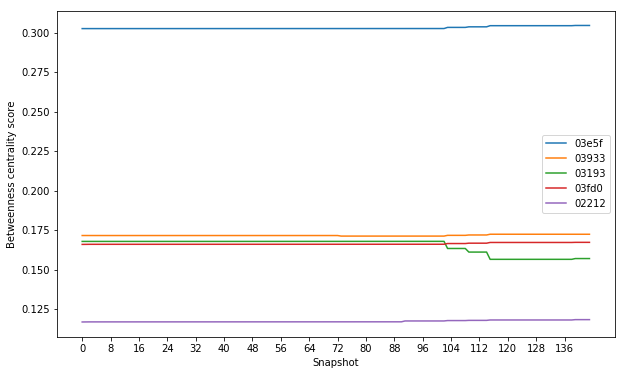
\includegraphics[width=\linewidth]{daily_betweenness_centrality1}
			\caption{Snapshot, May 21th}
			\label{daily_betweenness1}
		\end{subfigure}
		\begin{subfigure}{0.45\textwidth}
			\centering
			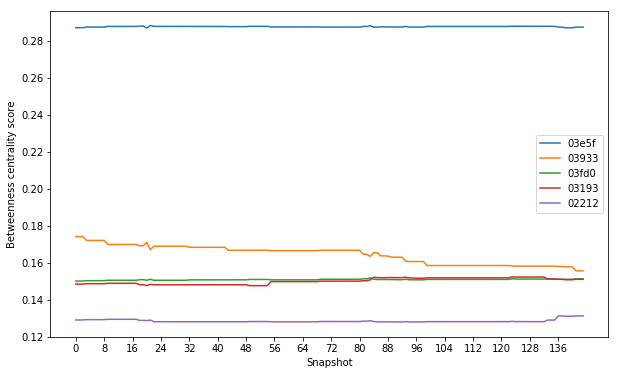
\includegraphics[width=\linewidth]{daily_betweenness_centrality2}
			\caption{Snapshot, May 26th}
			\label{daily_betweenness2}
		\end{subfigure}
		\begin{subfigure}{0.45\textwidth}
			\centering
			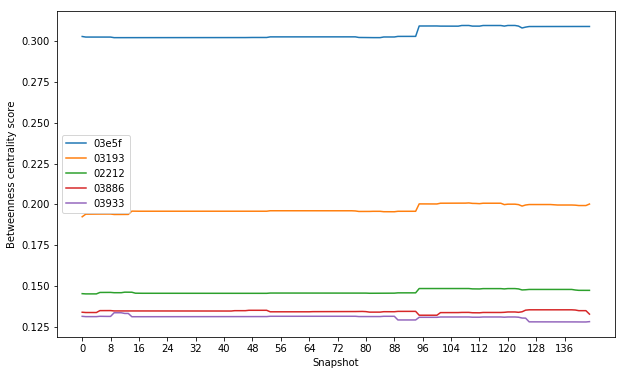
\includegraphics[width=\linewidth]{daily_betweenness_centrality3}
			\caption{Snapshot, June 2nd}
			\label{daily_betweenness3}
		\end{subfigure}
		
		\caption{Betweenness centrality}
		\label{daily_betweenness}
	\end{figure}	
	
	The data in Figure \ref{daily_betweenness} picks the top 5 nodes according to their betweenness centrality aggregated score. The aggregated score means that the centrality gets first evaluated for every node of the intersection $V = \{V_1 \cap V_2 \cap \cdots V_k \}$, where $k$ is the number of snapshot and $V_i$ being the set of nodes of each snapshot, then
	\begin{equation}\label{eq:betwenness}
		B_i(V) = \{ g_i(v) \mid \forall v \in V \}
	\end{equation}
	is computed, such that $B_i$ is the betweenness centrality score for all the nodes of the $i$-th snapshot. Then the nodes are sorted according to the aggregated score
	\begin{equation}
		B(V) = sort(\{ \sum_{j = 0}^{k}g_j(v) \mid g_j(v) \in B_i(V), \forall i= 0,1,2 \cdots k\})
	\end{equation}
	and the top five elements by score are picked otherwise it would be impossible to visually put in relation the betweenness centrality scores and the respective nodes. Also, computing the intersection between the set of nodes gives us the opportunity to speculate over a possible backbone structure composed by nodes with higher centrality score and to observe significant events occurred during an observation period over central players.
	
	As expected, the scores appear to be constant or with low variations along the 144 snapshots. The nodes are identified by the first five characters of their public key, and by looking at those IDs it emerges that the set is different for all their snapshot meaning that indeed new nodes joined the network during the five days elapsed between each snapshot and attached to already well established nodes. This aspect is even more pronounced if we look at Figure \ref{monthly_betweenness_centrality} where the monthly behavior is displayed and thanks to this metric is possible to investigate deeper on nodes and events that occurred during the observation period. 
	
	\begin{figure}[ht!]
		\centering
		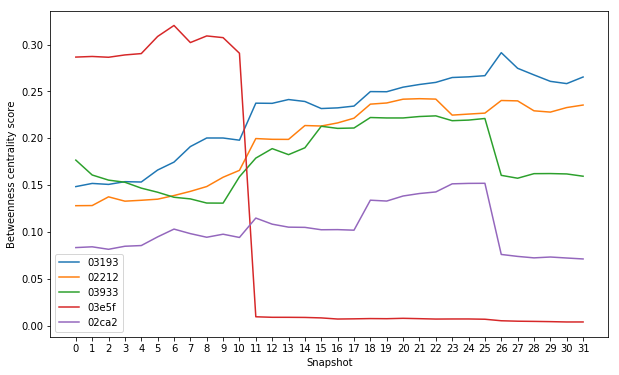
\includegraphics[width=\linewidth]{monthly_betweenness_centrality}
		\caption{Betweenness Centrality (Monthly)}
		\label{monthly_betweenness_centrality}
	\end{figure}		
	
	For example it has been noted that, on average, the total number of neighbors of these five nodes is 486.125, accounting for 62,7\% of the overall size of network. Such a high centrality score also suggests that a portion of neighbors may only have a single channel that keeps them connected to the rest of the network. To test this hypothesis we removed these five top nodes from the latest snapshot, and the result was that the graph got partitioned into 234 subgraphs: the largest subgraph among these contained 532 nodes (which is the Lightning Network itself) while the number of nodes of the remaining subgraphs is 242. Out of these 242 nodes, 228 were single channel nodes. However, given the nature of the network, disconnecting central nodes has no effect on the network connectivity as the giant connected component still remains connected.

	It is then possible to investigate over some peculiar events like the one happened during snapshot 10 and 11, where node \textit{03e5f9} lost suddenly its centrality over 24 hours: 
	from day 0 through day 10 the node was performing first among the others for betweenness centrality score. On day 11, the node dropped from 196 nodes to 37 as it closed channels with 159 peers; out of these 159 peers, 98 (12\% of the total nodes) of them were single channel nodes, effectively disconnecting them from the rest of the network. Unfortunately it's impossible to determine the causes that led to such a drop as it may be happened because of saturated channel balances, unresponsive nodes or internal errors on their server.
	
	\begin{figure}
		\centering
		\begin{subfigure}{0.8\textwidth}
			\centering
			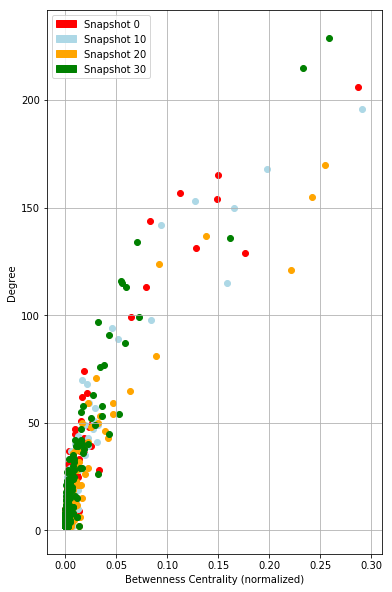
\includegraphics[height=0.8\linewidth]{scatter_plot_betweenness_centrality}
			\caption{normal scale}
		\end{subfigure}
		\begin{subfigure}{0.8\textwidth}
			\centering
			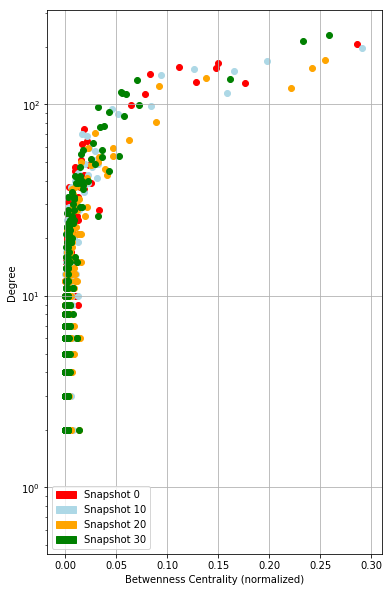
\includegraphics[height=0.8\linewidth]{scatter_plot_betweenness_centrality_semilog}
			\caption{semi-log scale}
		\end{subfigure}
		\caption{Betweenness centrality degree distribution in normal and semi-log plot with normalized betweenness centrality values. }
		\label{betweenness_centrality_degree}
	\end{figure}
	
	\subsection{Attack strategy on Betweenness Centrality}
	
	Cases like the one observed before suggest that in this network the more a node is connected towards single channel nodes (i.e. nodes with degree equals to 1), the more those nodes will be central since they will act as bridges for every single channel node that is connected to the rest of the network. Figure \ref{betweenness_centrality_degree} shows the relation between the normalized betweenness centrality score and the degree of each nodes for 4 different time instant of the graph (0, 10, 20, 30): the highest performing nodes are also the ones whose degree his higher as expected because they act as gateways for peripheral nodes. 
	
	The previous intuition gave us the opportunity to stress the network against an attack strategy based on the removal of central nodes. The focus in this work is on the effect of such an attack rather than the causes, so the attack here is carried under the assumption that every node of the network can be shut down at every instant. It is also worth to stress the fact that while we may hypothetically be able to provoke a DoS over nodes of the network, there's no way to enforce the closure of a channel except by forcing a node to stay offline until the time-lock of a Commitment Transaction runs off, that is because a channel is a cryptographically secure contract exclusively between two parties. The attack is performed by removing from the graph the node that scored the highest betweenness centrality value and all the nodes that got disconnected by such removal from the most connected component of the graph. Afterwards, the betweenness centrality is re-evaluated over the new graph and the process is iterated until there are no more nodes left to remove. 
	
	\begin{figure}[h]
		\centering
		\begin{subfigure}{0.45\textwidth}
			\centering
			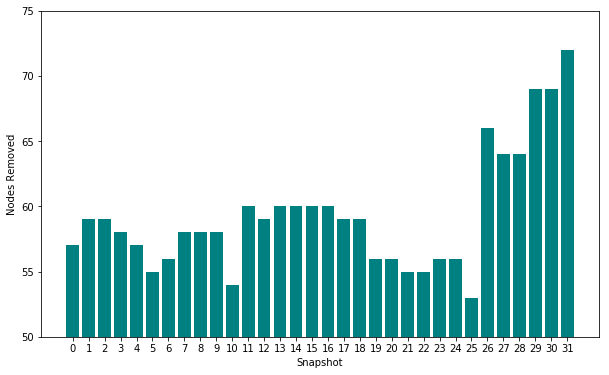
\includegraphics[width=\linewidth]{monthly_betweenness_centrality_attack}
			\caption{Number of nodes needed to disconnect the network}
		\end{subfigure}
		\begin{subfigure}{0.45\textwidth}
			\centering
			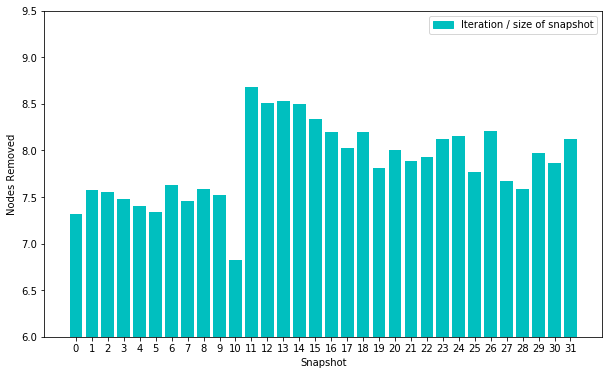
\includegraphics[width=\linewidth]{monthly_betweenness_centrality_attack_percentage}
			\caption{Percentage of nodes wrt graph size of current snapshot.}
		\end{subfigure}
		\caption{Number of iterations for each snapshot needed to disconnect every node of the network.}
		\label{betweenness_attack}
	\end{figure}
	
	The algorithm was performed over every snapshot of the network, and the result exceeded our optimistic previsions as the number of nodes required to completely destroy the network is fairly low compared to its size. Figure \ref{betweenness_attack} shows	how many iterations (i.e. nodes to be removed since every iteration removes at least one node) are needed to shut-down the network for each snapshot. The removal of a nodes produces many subgraphs whose size is usually 1, thus it's hard to determine a cut that produces large size partitions. Setting up and perform such an attack should be a feasible task: indeed, to the best of our knowledge, a successful DDoS attack has been already carried over the real network in March 2018, and resulted in 200 nodes disconnected from the network when the network size was of about 1000 nodes, thus disconnecting the 20\% of the clients which is actually higher than the average of 7.86\% of nodes found with this method. Details on this attack have not been revealed but is said to be leveraging on \textit{open-channel requests} in order to open as many TCP/IP connections as possible.
	
	By looking at the history of the betweenness centrality score is then possible to understand better the reliability of particular nodes, and to track nodes that get too centralized around hubs, thus making the network more and more similar to the current transaction processors like VISA or Mastercard: the autopilot feature of the Lightning Network might check the whole network betweenness centrality to regulate the new channels establishment process in order to decrease the centralization around greedy players. Another risk factor for centralization is given by the fact that central nodes are subjected to increased computational processing since each routed payment processed has a computational cost associated (albeit being low); collecting Lightning Network fees is less profitable than mining blocks, hence the need to maximize the earnings by reducing the operational costs in terms of energy spent, and this will likely force active members of the Lightning Network to opt for devices with lower performances: overloading such devices with routing tasks may drastically increase the fault probability, thus impacting on the overall network quality of life.
	
	\section{\textit{k}-vertex connectivity}

	\begin{figure}
		\centering
		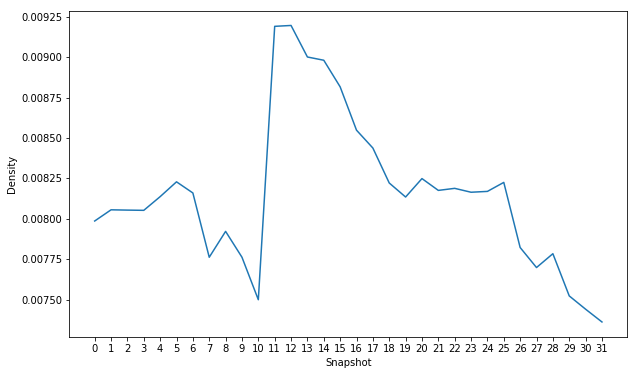
\includegraphics[width=\linewidth]{monthly_completeness}
		\caption{Density of the graphs. Density is calculated as $\frac{m}{n(n-1)}$}
		\label{monthly_completeness}
	\end{figure}
	
	\textit{k}-vertex connectivity gives an important outlook when it comes to robustness. In graph theory a graph $G = (V,E)$ is said to be \textit{k}-vertex connected if for every pair of vertices there are \textit{k}-vertex indipendent paths connecting these vertices, or in other words, \textit{k} is the size of the smallest subset of vertices such that the graph becomes disconnected if deleted. Complete graphs do not fall into this definition since a complete graph cannot be disconnected by removing vertices. Furthemore, if a complete graph has n-vertices, then by the above definition it falls in the class of (n-1)-vertex connectivity, but as Figure \ref{monthly_completeness} shows, the network is far to be complete.

	Computing the k-vertex connectivity alone over the snapshots is not particularly useful as the Lightning Network, being a connected network, will always be a 1-vertex connected graph. Nonetheless, it's very likely that inside the 1-vertex connected component there may be others, stronger, connected components, i.e. there may exists subgraphs whose k-vertex connectivities are higher than their supergraph. This kind of reasoning can be applied iteratively until it's impossible to find any new subgraph whose k-vertex connectivity is higher than their supergraph.
	
	The algorithm used to perform this task has been proposed by James Moody and Douglas R. White \cite{Moody2003} based on their research over cohesion in social groups. It returns the k-component structure of a graph G, where a k-component is a maximal subgraph of G that has at least node connectivity k. The algorithm works as follow:
	\begin{enumerate}
		\item Compute node connectivity k of the input graph.
		\item Identify all k-cutsets at the current level of connectivity. 
		\item Generate new graph components based on the removal of these cutsets. Nodes in a cutset belong to both sides of the induced cut.
		\item If the graph is neither complete nor trivial, return to 1; else end.
	\end{enumerate}
	
	The algorithm has been running over the 32 snapshots. What emerged is an inherent hierarchical structure of the network where the innermost components shows a high k-vertex connectivity (or cohesive degree) compared to the most peripheral nodes. Trivially, as the connectivity increases, the vulnerability to isolated actions performed unilaterally by some (byzantine) nodes decreases such that the degree of actions of any malicious attacker depends on at least $k$ components of the subgraph.
	
	\subsection{Components size}
	
	\begin{figure}[ht!]
		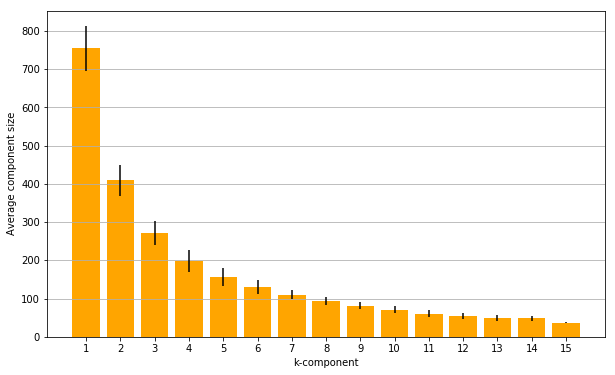
\includegraphics[width=\linewidth]{k_connectivity_average_size}\\
		\caption{Average size for each components for every snapshot taken from May 15th to June 27th}
		\label{monthly_connectivity_average}
	\end{figure}
	
	\begin{figure}
		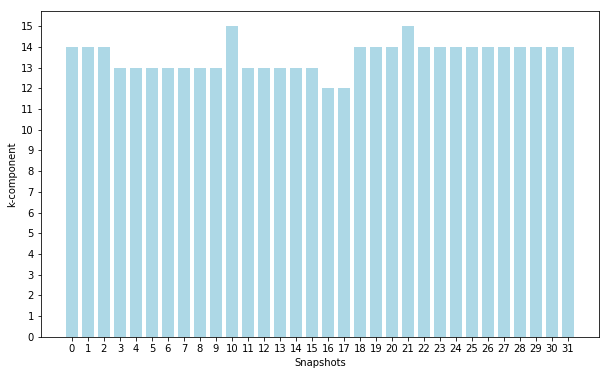
\includegraphics[width=\linewidth]{k_connectivity_max_size}
		\caption{Highest connectivity value for each snapshot.}
		\label{monthly_connectivity_max_size}
	\end{figure}
	
	The data presented in Figure \ref{monthly_connectivity_average} represents the average size of each component over the 32 snapshots in exam. The orange bars represent the mean value of every component while the black lines represent their standard deviation.	The 1-connected component is trivially the average of the graph sizes over the 32 captures; indeed every 1-connected component size is equal to the graph order of the relative snapshot. More than 50\% of the network is a biconnected subgraph (2-vertex connected graph) meaning that every node inside it is resilient up to two opportunely selected node failures (that is, nodes selected according to the well-known min-cut criteria) and, as we move right in the plot, the graphs get more and more resistant to node failures. What emerges from the analysis of the k-vertex-connectivity structure is a concentric configuration in which every k-component is included inside the (k-1)-component: this key aspect stresses the resilience to failures typical of scale-free networks as it would be impossible for attackers to disconnect a reasonable number of nodes in order to provoke any serious damage to the network. Figure \ref{monthly_connectivity_max_size} depicts the highest value k obtained for each snapshot and shows a dynamic behavior of k-connectivity, ranging from a lower bound of 12 to an upper bound of 15.
	
	\subsection{Betweenness inclusion}
	
	It is interesting to see which nodes belong to the top connected component. The intuition is that nodes that scored best in betweenness centrality will likely to belong to the highest k-component. The results were achieved in the following way:
	\begin{enumerate}
		\item Calculate $B_i(V)$ for each snapshot as seen in \ref{eq:betwenness}. Sort the result in a descending fashion. 
		\item For each $B_i(V)$ selects the first $s$ elements, where $s = |C_i|$ and $C_i$ being the set of nodes that belong to highest k-vertex component of the snapshot $i$.
		\item Compute the intersection between the two sets.
	\end{enumerate}
	
	\begin{figure}
		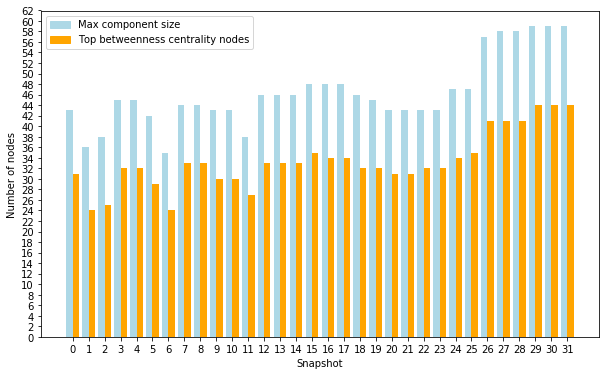
\includegraphics[width=\linewidth]{k_connectivity_beetwenness}
		\caption{Blue bars show the size of the maximum k-connected subgraph, orange bars show how many nodes selected among the top betweenness centrality nodes belong to the most connected component.}
		\label{monthyl_k_connectivity_betweenness}
	\end{figure}
	
	The results are showed in Figure \ref{monthyl_k_connectivity_betweenness} and as expected a large portion of the top performing central nodes are inside the innermost connected component. Data shows that on average the 72,34\% of the current top central nodes by betweenness centrality score belong to the most cohesive group of each snapshot.
	
	This aspect has several possible implications: as the network grows in size it will be unfeasible for each nodes to obtain and maintain the evolution of the whole network topology; a solution would be to organize the various Lightning Network nodes in a way similar to the Internet Network where backbone routers, which have a higher capacity, tie together various large subnetworks. Of course such a solution should be implemented according to the Bitcoin "no-trusted-third-parties" philosophy in mind. Central nodes inside this subgraph could be elected to actively participate in this backbone, and it is possible to extend this reasoning to lower k-connected components everytime the network grows in size to form a hierarchical structure as seen on computer networks. 
	
	The downsides in having so many central nodes tied together in such a strong connected component is that they may organize into cartels and decide to offer fast and reliable transaction processing only to nodes who adhere (by paying a fee or by submitting to some conditions) to their payment subnetwork while they act as gateways when it comes to route incoming and outgoing payments, in contrast with the decentralization principles of the network. Also such a scenario would suffer from low fairness with respect to transaction processing as they could refuse to process transaction that don't belong to their cartel.

	\section{Lightning Network as a Scale-free network}
	
	Many features that has been showed so far suggests that the Lightning Network is a complex network: the hierarchical fault tolerance showed in the k-vertex connectivity analysis, a high centrality of some high degree nodes making them hubs, the low diameter of the network compared to its number of nodes and edges are common features in scale-free networks. Such networks are random graphs whose degree distribution follows a power law such that 
	$$P(k) \sim k^{-\gamma}$$
	where $\gamma$ is a parameter whose value is usually $2 < \gamma < 3$. For this reason the degree distribution has been evaluated for all the snapshot of the period of observation. Given a graph $G = (V,E)$, $P(k)$ is defined as the probability for a node in V drawn at random of having exactly $k$ edges. Mathematically, it can be expressed as:
	$$P(k) = \frac{|\{ v_i \in V : \deg v_i = k \}}{|V|}$$
	where $k = \{0,1 ... n - 1\}$ and $n = |G|$. 
	
	\begin{figure}
	\centering
	\begin{subfigure}{\textwidth}
		\centering
		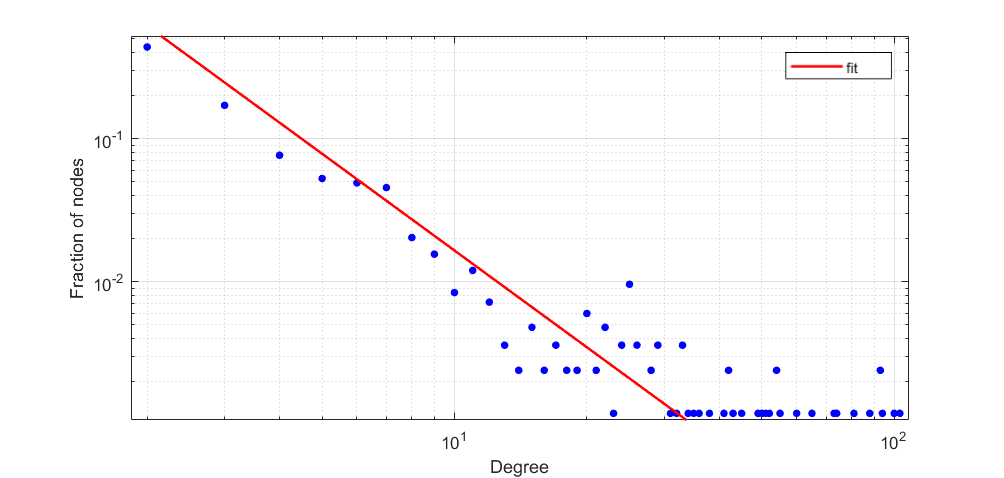
\includegraphics[width=\linewidth]{graph_28_scatter}
		\caption{log-log plot of the degree probability.}
		\label{graph_28_scatter}
	\end{subfigure}
	\begin{subfigure}{\textwidth}
		\centering
		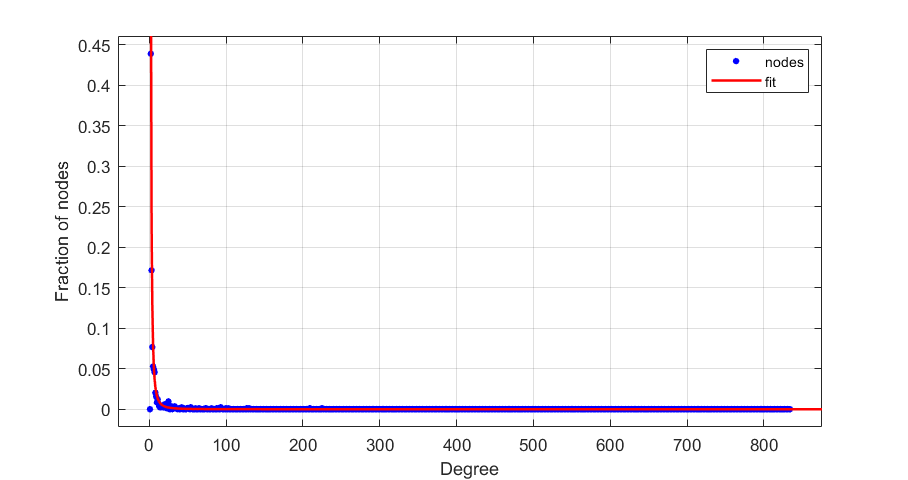
\includegraphics[width=\linewidth]{graph_28_fit}
		\caption{Curve fitting over the probability distribution.}
		\label{graph_28_degree}
	\end{subfigure}
		\caption{Degree distributions from snapshot 28 in log-log scale and standard scale}
	\end{figure}
	
	The autopilot feature of the Lightning Network shows a preference towards higher degree nodes when it comes to open new payment channels and indeed it uses the Barabàsi-Albert model preferential attachment to perform this task, which assumes $\gamma=3$ for the degree distribution. However, many nodes of the real network are configured to custom parameters such as the maximum number of channels allowed, therefore introducing a bias in the network structure that makes the system diverge from the ideal representation. It is of interest then to compare different models based on a power-law distribution to see which one fits better the nature of the network. Thus, the first attempt was to generate a new network using the BA-model with 886 nodes and 2649 edges, which is the maximum size of the Lightning Network encountered so far. This will later be put in comparison to another power-law model.
	
	In order to build a graph that responds to a power-law degree distribution, it is necessary to first figure out the value of $\gamma$ from the data gathered so far using the definition of degree distribution $P(k)$ shown above. For the sake of clarity, Figure \ref{graph_28_scatter} and \ref{graph_28_degree} shows the degree distribution for a single capture of the graph, in a log-log and normal scale respectively. Unfortunately since the adoption of the network is still low and because the network has been studied on the testnet environment due to size constraints, the amount of data results to be scarce and many outliers occur. As a consequence it has been chosen to use the Bisquare weights regression where weight is given to each data point based on how far the point sits from the fitted curve, thus minimizing the effect of outliers points.
	
	By using the curve fit tool from Matlab, it has been possible to evaluate the gamma value of the fitting curve for each snapshot such that $\Gamma = \{\gamma_1, \gamma_2, ... , \gamma_d\}$ where $d$ is the number of snapshots, using Bisquare as robust regression and the Trust-Region algorithm, then mean, variance and standard deviation has been evaluated over $\Gamma$.
	
	\begin{center}
		\begin{tabulary}{0.75\linewidth}{| L | C | C | C | }
			\hline
			& Mean & Variance & Standard Deviation \\ \hline
			$\gamma$ & 2.0453 & 0.226 & 0.1503  \\ \hline
		\end{tabulary}
	\end{center}
	
	
	From the $\gamma$ value, a new graph has been created with a number of nodes in the order of the sizes seen until now, specifically 886 nodes as it has been done with the BA-model: firstly, a degree sequence that follows a power-law distribution with a given exponent has been calculated, then the graph was generated through an algorithm modeled around the preferential attachment property of scale-free networks by W. Aiello, F. Chung and L. Lu, \cite{Aiello2001} \cite{Chung2002}, which performed best with respect to the \textit{configuration model} from M. Newman \cite{Newman2003}, where graphs with self-loops and parallel edges are a possible outcome of the generative process; manually removing these would cause an important structural bias. The Chung-Lu generative approach doesn't explain why a graph has a particular degree sequence, rather, this model tries to derive the structural properties of a real network, starting from a power-law degree sequence.
	
	The features we are interested in are the one that describe the topology of a graph. Because of the random generative process, the data here showed is the average results for each metric gathered by 100 random graphs generated by the BA and Chung-Lu models. An important aspect of scale-free networks is the \textit{small world} property, where a network is said to be a small world if its diameter is low compared to the total number of nodes. It has already been observed that the current diameter for the Lightning Network is around 7 and 8; results on the generated networks still carries this aspect, as showed on the table below.
	
	\begin{center}
		\begin{tabulary}{\linewidth}{| C | C | C | C | C |}
			\hline
			& Radius & Diameter & Eccentricity & Shortest Path \\ \hline
			Real World & 4.0 & 7.656 & 5.50 & 3.098 \\ \hline
			Chung-Lu model & 3.48 & 6.54 &  4.778 &  2.719 \\ \hline
			BA-model & 3.87 & 6 & 4.9188 & 3.487 \\ 
			\hline
		\end{tabulary}
	\end{center}
	The eccentricity and diameters value of the two models here are almost identical, with the Chung-Lu model performing slightly better than the BA-model which shows a shorter diameter but a higher average shortest path length.
	
	Another good metric for comparing different networks is the average clustering coefficient, which is a way to measure how close a node and its neighbors are to being a clique and it's defined for undirected graph for every node $i$ of the graph as $$C_i = \frac{\lambda_G(v)}{\tau_G(v)}$$ where $\lambda_G(v)$ is the number of subgraphs of the graph with 3 vertices (one of which must be $v$) and 3 edges, and $\tau_G(v)$ is the number of triples, i.e. the number of subgraphs with 3 vertices and 2 edges, in which $v$ is incident to both the edges. The table below shows the results for the real network, the network generated through Chung-Lu algorithm and the BA model.
	\begin{center}
		\begin{tabulary}{0.75\linewidth}{| C | C |}
			\hline
			& Average Clustering Coefficient \\ \hline
			Real World & 0.20591 \\ \hline
			Chung-Lu model & 0.3368 \\ \hline
			BA-model & 0.03322 \\
			\hline
		\end{tabulary}
	\end{center}

	Here the differences between the two models are more pronounced. While the Chung-Lu model shows an average clustering coefficient in line with the real case scenario, the BA-model lacks on catching properly the aspect of centralized hubs which are a fundamental characteristic of the Lightning Network. Furthermore, this aspect is also reflected by degree distribution in relation to the betweenness centrality that we already seen in Section \ref{sec:betweenness}. Figure \ref{betweenness_centrality_degree_models} shows degree betweenness centrality distributions of two random generated graphs both in linear and semilogarithmic scale. What emerges is that the betweenness score from BA-model is quite lower than the Chung-Lu and real network, and this was kinda expected given the that the average clustering coefficient has been shown to be low, suggesting that nodes in BA do not model the central hubs as well as in Chung-Lu.
	
	\begin{figure}[]
		\centering
		\begin{subfigure}{0.49\textwidth}
			\centering
			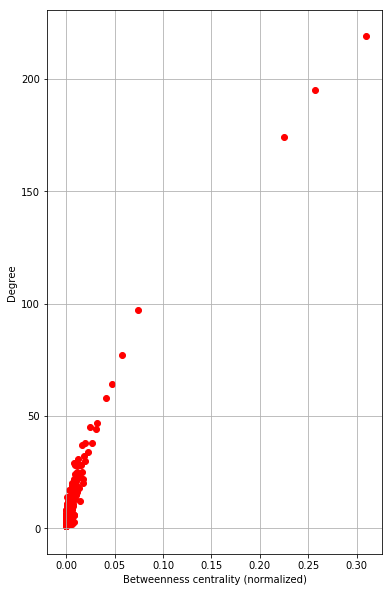
\includegraphics[width=\linewidth]{scatter_plot_betweenness_centrality_chung_lu}
			\caption{Chung-Lu model}
		\end{subfigure}
		\begin{subfigure}{0.49\textwidth}
			\centering
			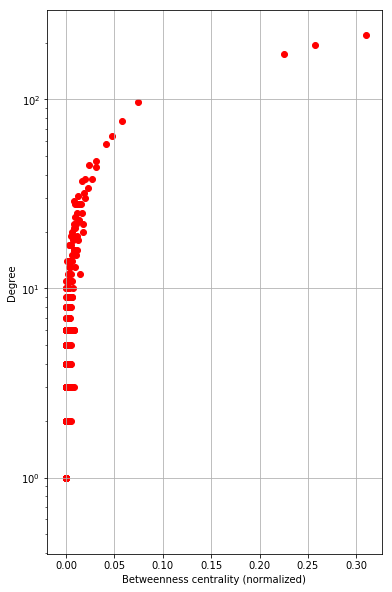
\includegraphics[width=\linewidth]{scatter_plot_betweenness_centrality_chung_lu_semilog}
			\caption{Chung-Lu model (semilog)}
		\end{subfigure}
	
		\begin{subfigure}{0.49\textwidth}
			\centering
			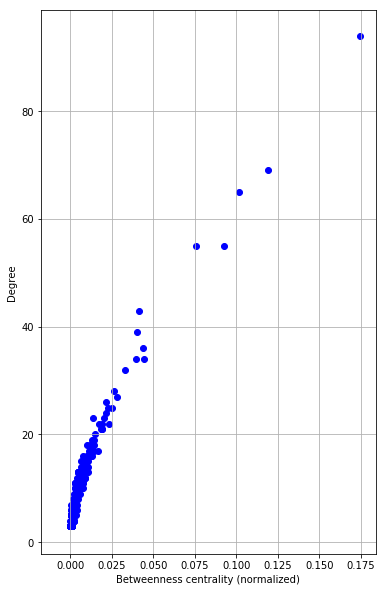
\includegraphics[width=\linewidth]{scatter_plot_betweenness_centrality_barabasi}
			\caption{BA model}
		\end{subfigure}
		\begin{subfigure}{0.49\textwidth}
			\centering
			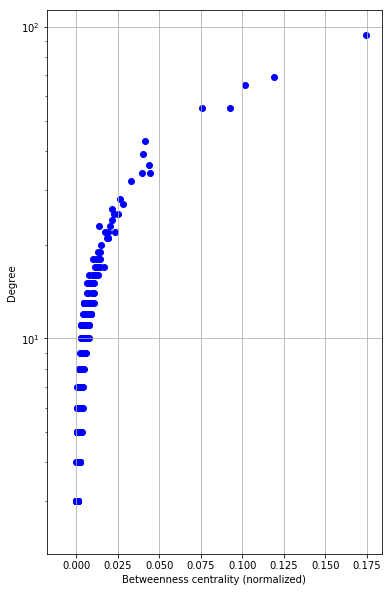
\includegraphics[width=\linewidth]{scatter_plot_betweenness_centrality_barabasi_semilog}
			\caption{BA model (semilog)}
		\end{subfigure}
		\caption{Betweenness centrality degree distribution for BA and Chung-Lu generated networks.}
		\label{betweenness_centrality_degree_models}
	\end{figure}
	
	As already stated in \cite{Watts1998}, random graphs clustering coefficients are usually smaller with respect to real network ones because of the inability to describe at best the inevitable unpredictability of some phenomena. Hence a deeper understanding of the probability distribution with the exact $\gamma$ value was necessary to obtain an equivalent model able to show the same behavior of the real network.
	
	With this in mind, it's possible then to generate equivalent models of desired sizes based on the Chung-Lu generative approach, that has been showed to fit better with respect to the BA-model. As the size grows, the properties showed so far grow accordingly to the nature of the network. Testing the generated model against 10'000 nodes produced very interesting results, reported in the table below. Like before, the generated graph produced many isolated nodes and small size components, so it has been necessary to prepare the network  by removing these unnecessary entities before running the evaluation.
	
	\begin{center}
		\begin{tabulary} {\linewidth}{| C | C | C | C | C |}
			\hline
			Num. of nodes & Num. of edges & Clustering Coefficient & Diameter & Avg. shortest path \\ \hline
			8420 & 29969 & 0.1038 & 9 & 3.4679\\ \hline
		\end{tabulary}
	\end{center} 
	
	Results show a decreased average clustering coefficient, as the scale-free networks are supposed to perform when they grow in size, and overall the other parameters are in line with the values observed in the real network. It must be reminded however that data are based over the Testnet environment: unfortunately, generating an equivalent network for the Main-Net has been showed to be not accurate, as the average degree of the Main-Net appears to be higher than the one presented here, therefore the $\gamma$ value discovered so far is only representative of the testing network. However, the methodologies here presented are compatible with the real network environment so it should not be hard to see if they applies for a real world scenario.

	\section{Addressing node dynamicity}
	
	
	We introduce a formalism to describe the dynamic behavior of the network from nodes and edges points of view. The network evolution is described in a time interval defined as a set of integer $\{t_0, t_1, t_2 .... t_k \}$. Since the network was observed at fixed time interval  we can assume that for $\forall \: 0 < i \leq k,\: t_i-t_{i-1} = c$ and specifically in this work $c = 1$, hence we can refer to each time instant either by $t_i$ or its integer $i$ without loss of generality. For every time instant $t$, there is a graph $G_{t}= (V_t,E_t)$ where $V_t$ and $E_t$ represents the set of nodes and edges at time $t$ respectively. Nodes that constantly enter and leave the network are called \textit{churning nodes}. To characterize these two behaviors with respect to the time parameter we define two functions:
	\begin{definition}
		Join function. $\lambda(t)$ is defined as a discrete time, deterministic function that returns the number of nodes that joined the network at time $t$, i.e. they opened a payment channel with \textit{at least} one node of the network.
	\end{definition}
	\begin{definition}
		Leave function. $\mu(t)$ is defined as a discrete time, deterministic function that returns the number of nodes that left the network at time $t$, i.e. they closed \textit{every} payment channel with previously connected nodes.
	\end{definition}
	The join and leave rate has been evaluated through set differences between the vertices V of the various instance of the network such that
	$$\lambda(t_i) = |V_{t_i} \setminus V_{t_{i-1}}|$$
	$$\mu(t_i) = |V_{t_{i-1}} \setminus V_{t_i}| $$
	For initial time $t_0$ and for every $t \leq t_0$ the two functions returns 0.
	\begin{figure}[h]
		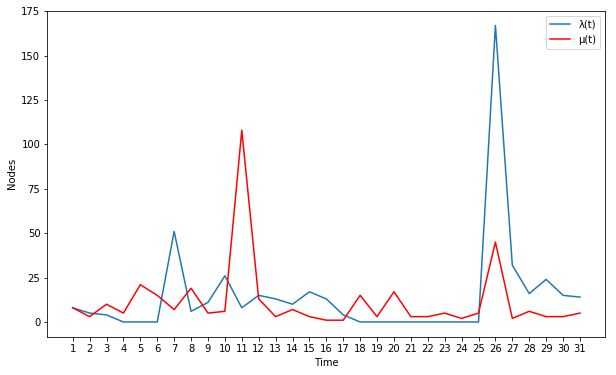
\includegraphics[width=\linewidth]{churn}
		\caption{$\lambda(t)$ and $\mu(t)$ functions over the observed time interval}
		\label{churn}
	\end{figure}
	\begin{figure}
		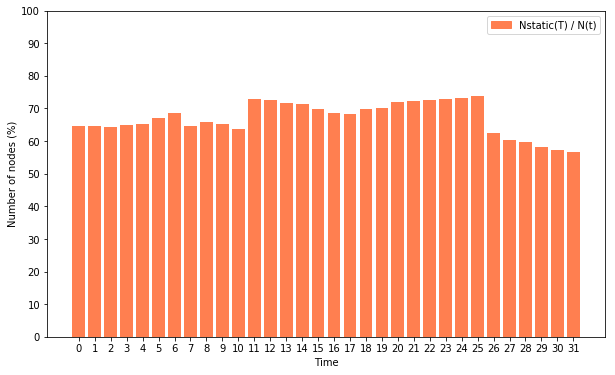
\includegraphics[width=\linewidth]{percentage_static_nodes}
		\caption{Percentage of stable nodes inside each $G_t$.}
		\label{percentage_static_nodes}
	\end{figure}
	Figure \ref{churn} shows the observed churn rates along the period of observation, putting in evidence a relatively small churning rates with respect to the number of nodes of each snapshot as previously displayed by Figure \ref{monthly_nodes}.
	
	If $\lambda(t)$, $\mu(t)$ and $N(t_0)$ are known, with $N(t_0)$ being the number of nodes at time $t_0$, it is then possible to know the size of the network thanks to
	\begin{definition}
		Nodes function. Let $N(t_0) = n_0$, the nodes function returns the number of nodes belonging to the system at time $t$ for every $t \geq t_0$, such that 
		$$N(t_0) = n_0$$
		$$N(t) = N(t-1) + \lambda(t) - \mu(t)$$
	\end{definition}
	We can proceed to calculate the actual churn rate of the network through
	\begin{definition}
		Join churn rate. Let $T = t_k - t_0$ being the interval of observation. The join churn rate is defined as
		$$\lambda_{rate} = \frac{\sum_{i = 1}^{k}\frac{\lambda(t_i)}{N_{t_i}}}{k},$$
	\end{definition} 
	\begin{definition}
		Leave churn rate. Let $T = t_k - t_0$ being the interval of observation. The leave churn rate is defined as
		$$\mu_{rate} = \frac{\sum_{i = 1}^{k}\frac{\lambda(t_i)}{N_{t_{i}}}}{k}.$$
	\end{definition}

	Data shows a modest churn rate being it $\lambda_{rate}=1.87\%$ and
	$\lambda_{rate}=1.51\%$. The largest portion of the network has been observed to be stable throughout the entire time interval. The static nodes of the Lightning Network have been evaluated by computing the intersection between the vertices of the various graph $G_t$, such that
	$$N_{static}(T) = |V_{t_0} \cap V_{t_1} \cap V_{t_2} ... \cap V_{t_k}|$$
	with $T = t_k - t_0$, defined as the interval of observation.
	
	The size has been found to be $N_{static} = 503$ nodes and Figure \ref{percentage_static_nodes} shows the fraction of nodes that are stable with respect to the total number of nodes for each graph $G_t$ but results may be skewed by two particular event as observed in Figure \ref{churn}, where we can first appreciate a severe drop in $\mu(t_{11})$, and that has already been addressed in Section \ref{sec:betweenness} where we commented on the behavior of the most central node shutting down 159 channels, and second, in $\lambda(t_{26})$, where 167 new nodes joined the network; the unexpected churn can be explained by a real fact that happened during the observation period where a user tried and succeeded to become the most important node per capacity score in the main-net environment in July 2018\footnote{https://medium.com/andreas-tries-blockchain/bitcoin-lightning-network-1-can-i-compile-and-run-a-node-cd3138c68c15}, so it is plausible that he performed some test over the testing environment before approaching the real network.
	
	\begin{figure}[h]
		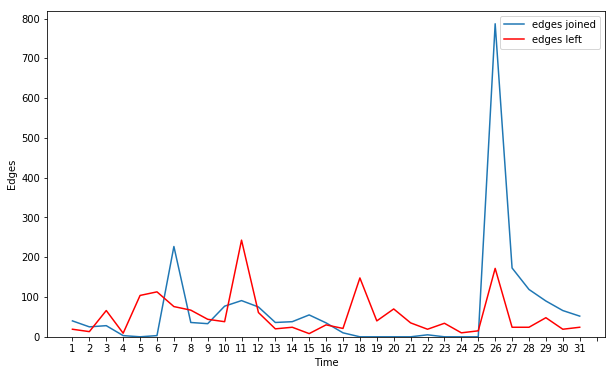
\includegraphics[width=\linewidth]{edge_churn_plot}
		\caption{Edges join and leave variation.}
		\label{fig:edge_churn}
	\end{figure}

	\begin{figure}[t]
		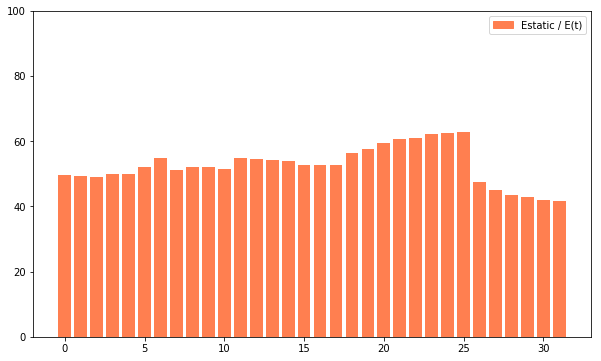
\includegraphics[width=\linewidth]{edge_stable_ratio}
		\caption{Static edges and number of edges per snapshot ratio.}
		\label{fig:edge_stable_ratio}
	\end{figure}
	
	\section{Addressing edge dynamicity}
	
	As more and more nodes join and leave the network, the channel structures changes accordingly (Figure \ref{fig:edge_churn}) with new channels being opened and closed between nodes. The network is characterized by a stable edge component that accounts for $E_{static} = 1202$ nodes and Figure \ref{fig:edge_stable_ratio} shows that, on average,  only 52.55\% of the edges of each snapshot are going to stay through all the observation period.	To better capture the dynamic behavior of the network, we introduce a formalism that takes into account the edge variability of a graph with respect to time. This framework is known as TVG or Time Varying Graph, and it is a unified model which is the integration of various existing models and concepts proposed in the literature for dynamic graphs. \\
	We define our TVG as a directed graph $\mathcal{G} = (V, E, \mathcal{T}, \rho, \mathcal{C}, A)$ where:
	\begin{itemize}
		\item $V$ and $E$ are the set of nodes of our network respectively. 
		\item $E: V \times V$ and each edge has a set of attributes $A(e) = [k_1(e),\, k_2(e)]$ which maps to <\textit{balance, htlc}> which is the htlc and balance value for node $i$. $A$ is a matrix of attributes accounting for every edge in $\mathcal{G}$.
		\item $\mathcal{T} \subset \mathbb{T}$ is the lifetime of the model.
		\item $\rho$ is the edge presence function such that $\rho: E \times \mathcal{T} \to \{0,1\}$.
		\item $\mathcal{C}$ is the set of channels: a channel $c_{u,v} = c_{v,u}$ between two nodes $u$ and $v$, is represented as two edges $e_{u,v}$ and $e_{v,u}$ such that $c_{u,v} = (e_{u,v}, e_{v,u})$. Furthermore, an edge $e_{ij}$ from node $i$ to $j$ exists iff there is an edge $e_{ji}$  from node $j$ to $i$.
	\end{itemize}
	
	The channel capacity is defined as $cap_{c_{u,v}} = k_1(e_{u,v}) + k_1(e_{v,u})$ and its constant through all the life window of the channel.
	The Time Varying Graph takes place on the \textit{lifespan} $\mathcal{T}  \subset \mathbb{T}$ where the domain of $\mathbb{T}$ is assumed to be $\mathbb{N}$, i.e. the system is discrete-time,and the underlying graph $G = (V, E)$ represents a \textit{footprint} of the graph in which the time aspect of a node is flatten out. 
	
	From a graph-centric point of view the evolution of $\mathcal{G}$ is described as a sequence of graphs $\mathcal{S}_{\mathcal{G}} = G_1, G_2, ... $ where a graph $G_i$ can be seen as a static snapshot of $\mathcal{G}$ at time $t_i$ and it is easy to see how this model perfectly fits with the data collected for this work, where each characteristic graph of $\mathcal{S}_{\mathcal{G}}$ corresponds to the snapshots observed so far. The power of expressiveness of this model resides on the fact that the granularity in which edges appear in the network can be adjusted in order to provide a more punctual information over the dynamic topology of the network: for example we could see how the model evolves when each time instant is considered to be 10 minutes, 30 minutes or 24 hours.

	In this model we addressed the problem of performing payments in the worst scenario (i.e. nodes uncooperative until payment expiration). We define an uncooperative payment function as follows:
	\begin{definition}
		\textit{uncooperativePayment}(u,v,s). Defines a payment function. A payment can be performed at time instant $t_n$ if:
		\begin{itemize}
			
			\item $\exists$ a path between node $u$ and $v$, denoted as $\pi =  \{c_{u,1} ... {c_{i,v}}\}$.
			\item $\forall$ edges $e$ in $\pi$ that connects $u$ to $v$, $k_{tot} = \sum_{e} k_2(e)$ such that $\rho(e, t_{n+i}) = 1, \, \forall n < i < n + k_{tot}$, that is a path must remain open for the duration of the payment.
			\item $\forall$ edges $e$ in $\pi$ that connects $u$ to $v$, $k_1(e) >= s$, i.e. an edge carries enough funds to allow the transfer of money.
			\item For every payment operation $\pi_i$ that is taking place in any instant between $[t_n, t_{n + k_{tot}})$ it must hold that $\pi \cap \pi_i = \emptyset$, meaning that there can't be two or more payments occurring on any edges that belong to $\pi$.
			\item at the end of the payment, $\forall$ edges $e_{ij}$ in $\pi$ that connects $u$ to $v$ it must hold that $cap_{i,j} = k_1(e_{i,j}) + k_1(e_{j,i})$ and $k_1(e_{j,i}) = cap_{i,j} - (k_1(e_{i,j}) - s)$.
		\end{itemize}
	\end{definition}

	The cooperative payment scenario between $u$ and $v$ can be modeled trivially by requiring $\forall$ edge $e$ that participates to the payment path $\pi$ to have at time $t_n$ $\rho(e, t_n) = 1$. The payment is resolved instantly and each channel from $u$ to $v$ updates its balance according to the amount of money transferred. 
	
	

\end{document}